%----------------------------------------------------------------------------
\appendix
%----------------------------------------------------------------------------
\chapter*{F�ggel�k}\addcontentsline{toc}{chapter}{F�ggel�k}
\setcounter{chapter}{6}  % a fofejezet-szamlalo az angol ABC 6. betuje (F) lesz
\setcounter{equation}{0} % a fofejezet-szamlalo az angol ABC 6. betuje (F) lesz
\numberwithin{equation}{section}
\numberwithin{figure}{section}
\numberwithin{lstlisting}{section}
%\numberwithin{tabular}{section}


\section{Az eredeti 1581-es floppy meghajt� kapcsol�si rajza}
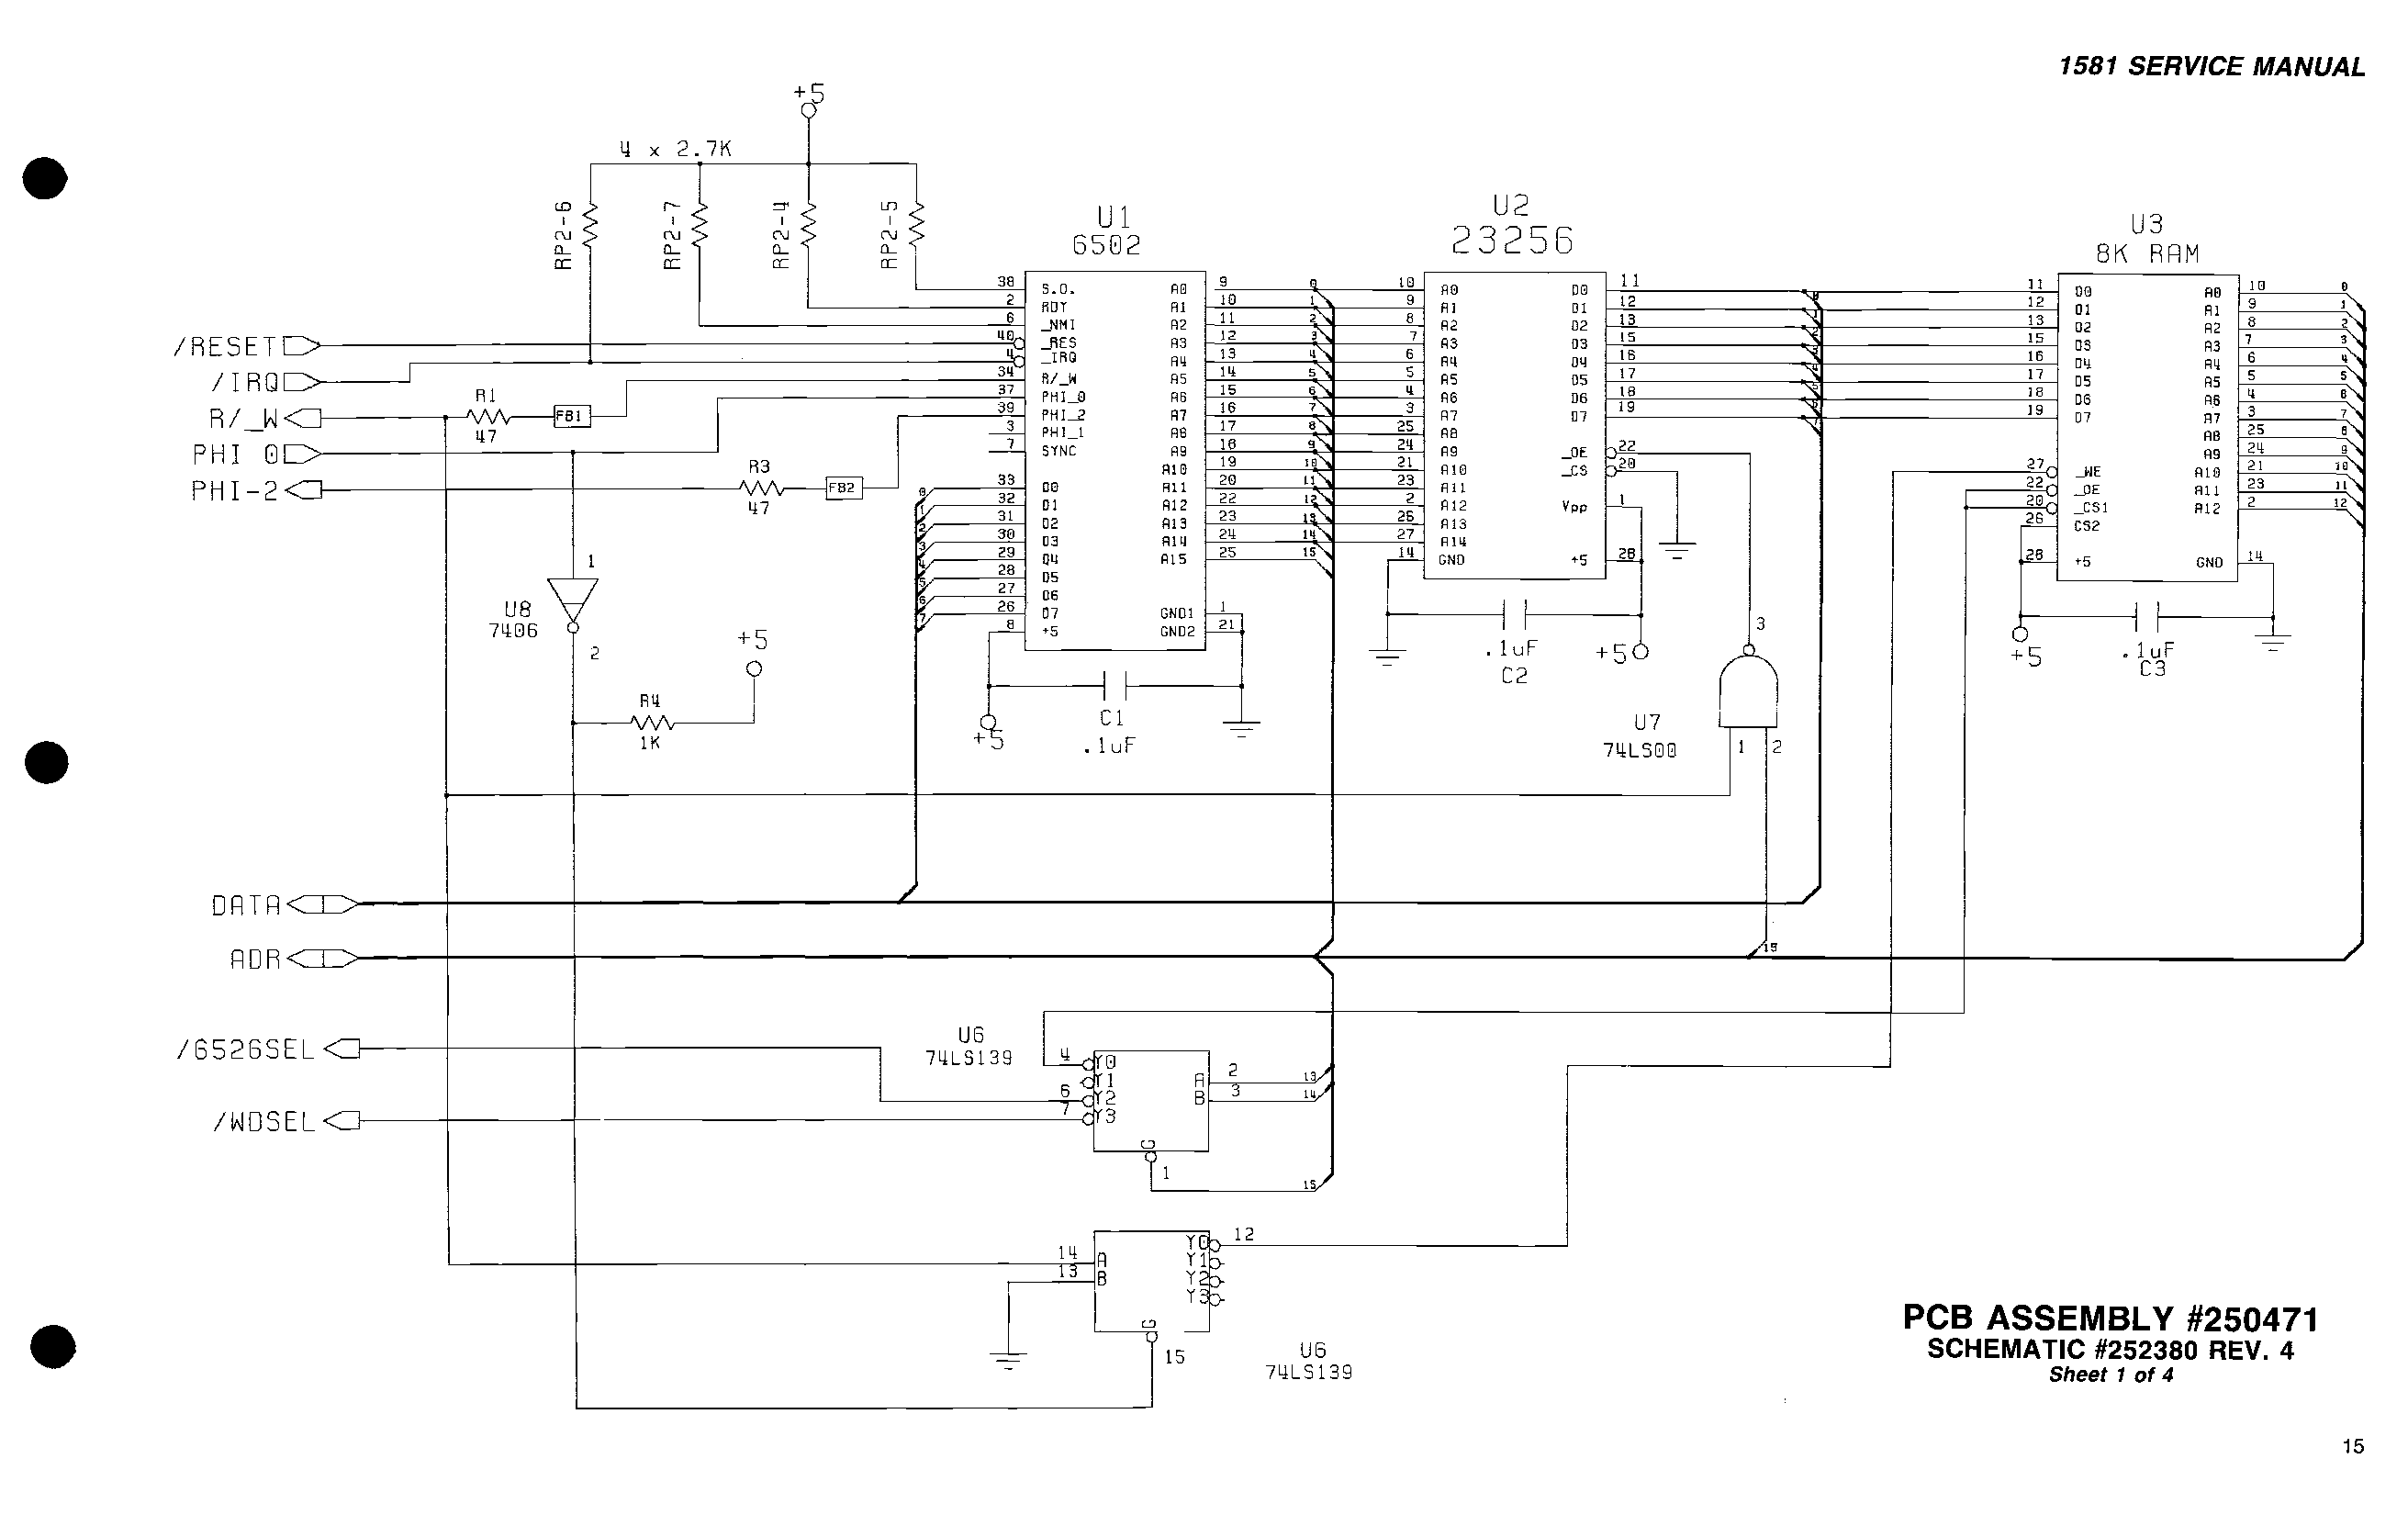
\includepdf[pages=-,angle=90]{appendices/1581_schematic.pdf}

\section{Az interf�szk�rtya kapcsol�si rajza}
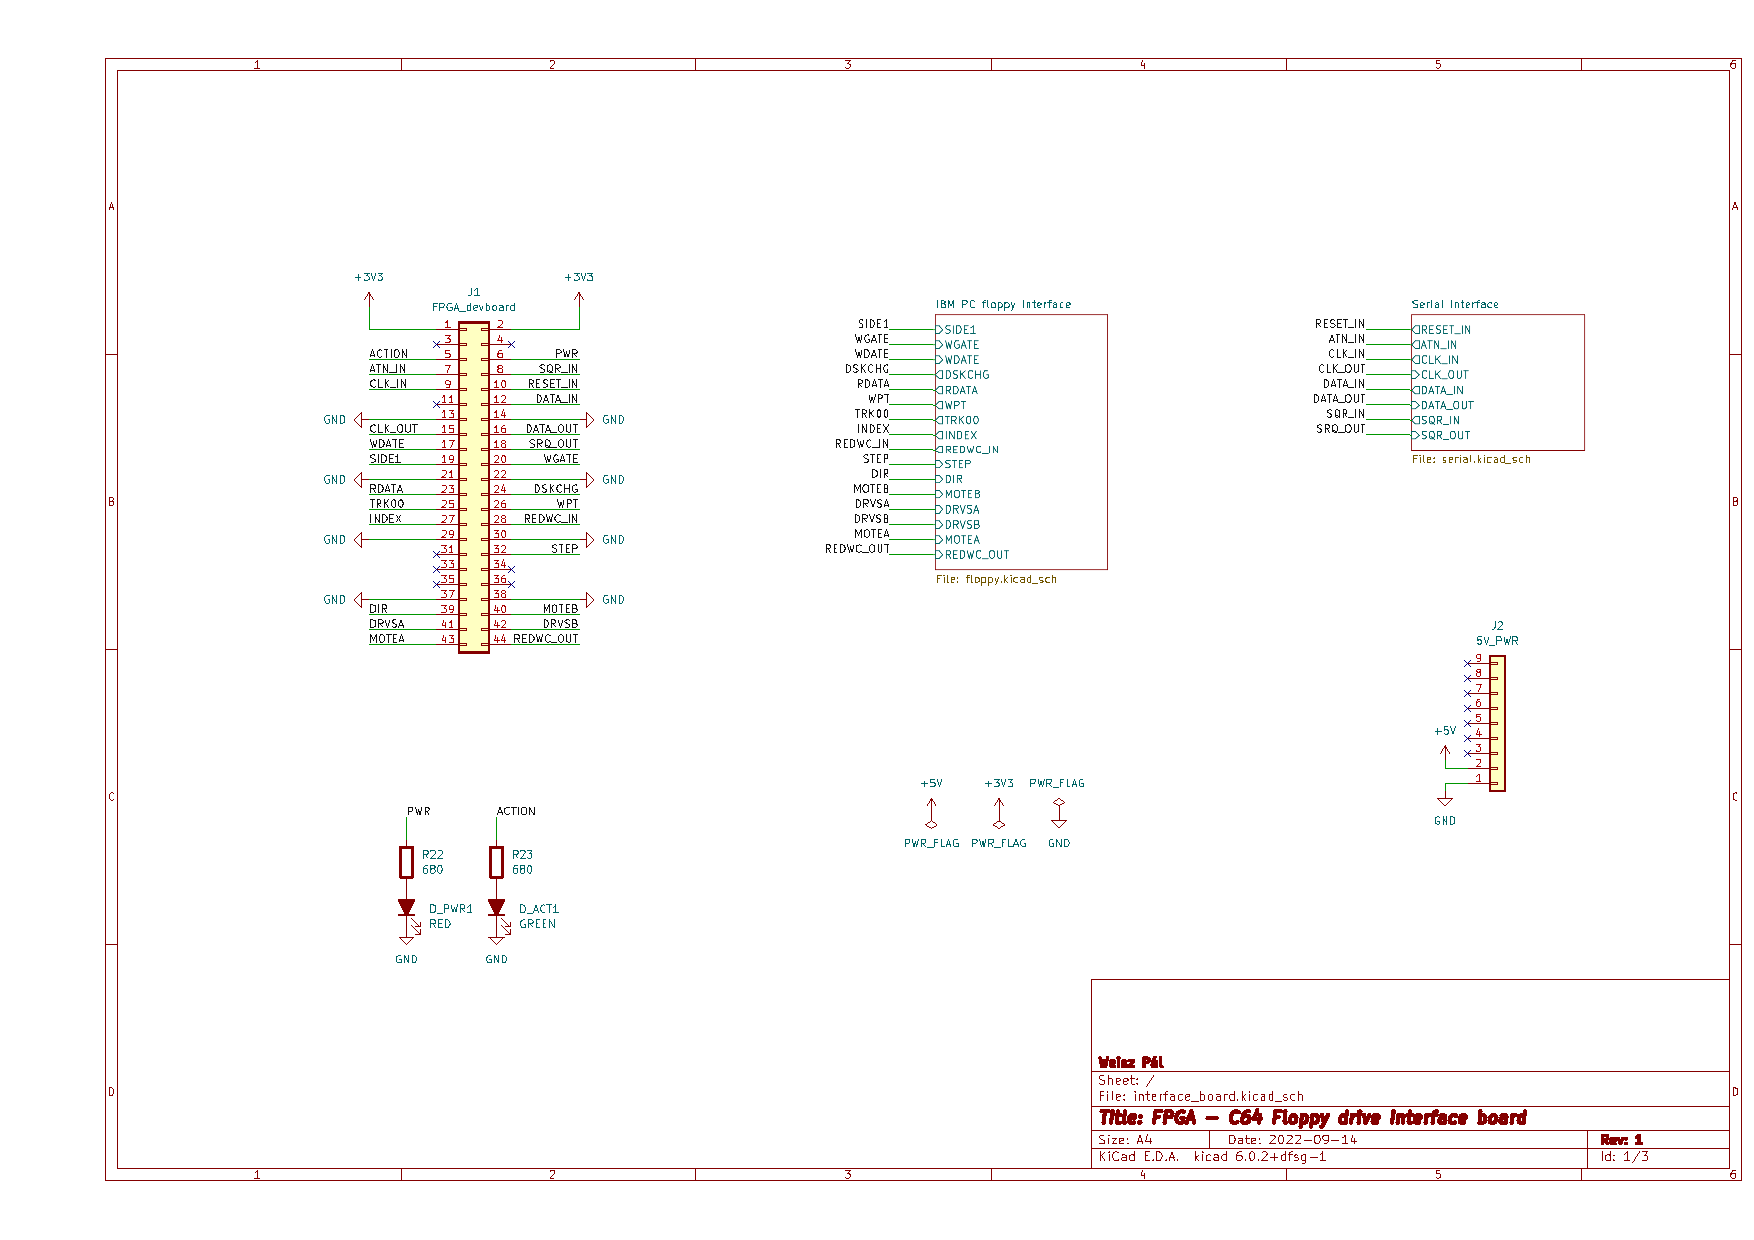
\includepdf[pages={-},angle=90, offset=0 -25]{appendices/interface_board.pdf}

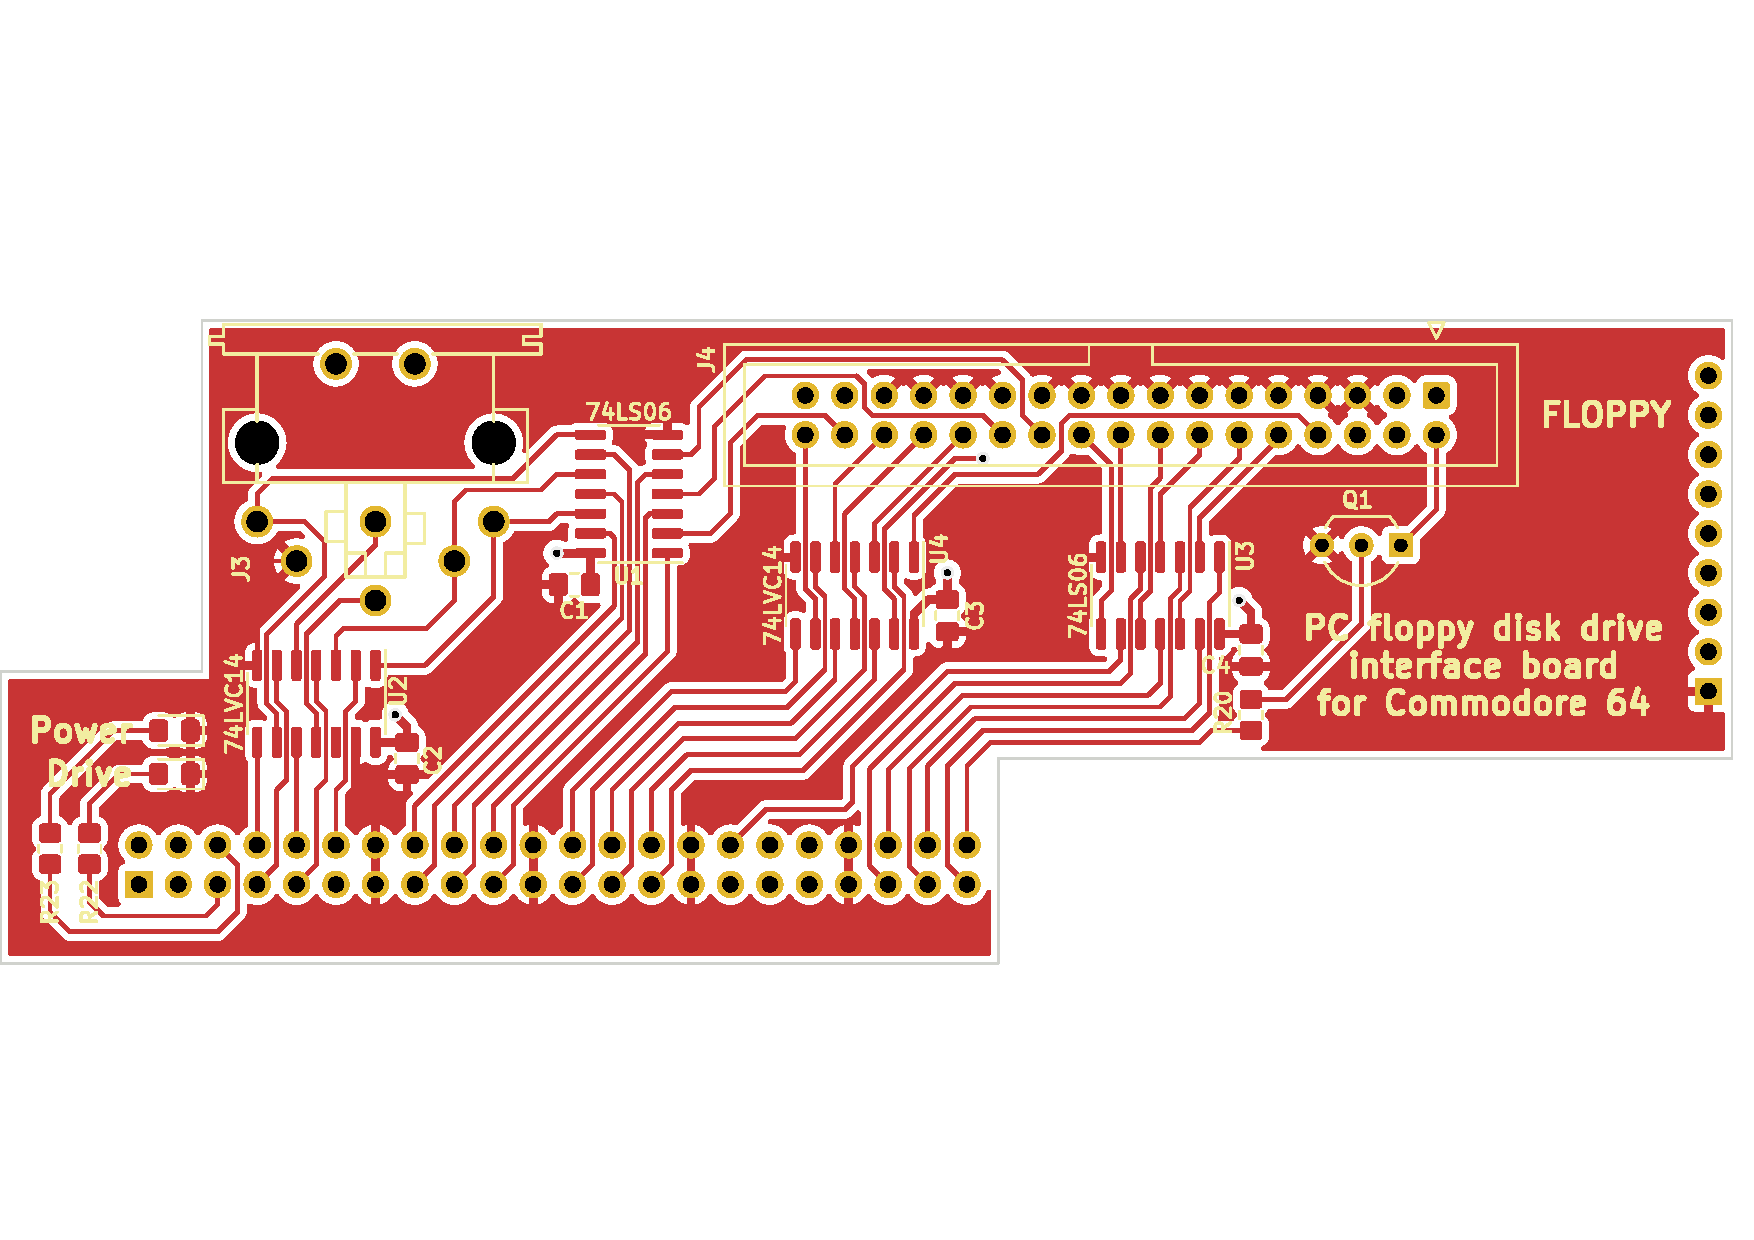
\includepdf[pages={-}, nup=1x2, scale=.8, pagecommand={\section{Az interf�szk�rtya NY�K-terve}}]{appendices/pcb.pdf}
